%
% Tesi D.S.I. - modello preso da
% Stanford University PhD thesis style -- modifications to the report style
%
%%%%%%%%%%%%%%%%%%%%%%%%%%%%%%%%%%%%%%%%%%%%%%%%%%%%%%%%%%%%%%%%%%%%%%%%%%%
%                                                                         %
%			TESI DOTTORATO                                                   %
%			______________                                                   %
%                                                                         %
%			AUTORE: Elena Pagani                                             %
%                                                                         %
%			Ultima revisione: 7.X.1998                                       %
%           correzioni atrent                                             %
%%%%%%%%%%%%%%%%%%%%%%%%%%%%%%%%%%%%%%%%%%%%%%%%%%%%%%%%%%%%%%%%%%%%%%%%%%%
%
%
\documentclass[a4paper,12pt]{report}
%\renewcommand{\baselinestretch}{1.6}      % interline spacing
%
% \includeonly{}
%
%			PREAMBOLO
%
\usepackage[a4paper]{geometry}
\usepackage{amssymb,amsmath,amsthm}
\usepackage{graphicx}
\usepackage{url}
\usepackage{epsfig}
\usepackage[italian]{babel}
\usepackage{setspace}
\usepackage{tesi}
\usepackage{nameref}
\usepackage[italian]{varioref}
\usepackage{footnotebackref}
\usepackage{hyperref}
\usepackage{caption}
\usepackage{subcaption}
\usepackage{pgfplots}
\usepackage{tikz}
\usepgfplotslibrary{fillbetween}
\pgfplotsset{width=10cm,compat=1.9}


% \captionsetup{width=1\textwidth,font={small, sl},labelfont={bf}}


% per le accentate
\usepackage[utf8]{inputenc}
% \graphicspath{.\Images}
%
\newtheorem{myteor}{Teorema}[section]
%
\newenvironment{teor}{\begin{myteor}\sl}{\end{myteor}}
%
%
%			TITOLO
%
% \includegraphics{Logo}
\begin{document}
\title{Implementazione e confronto di algoritmi di ottimizzazione per l'apprendimento di insiemi fuzzy}
\author{Giacomo Intagliata}
\dept{Corso di Laurea Triennale in Informatica} 
\anno{2020-2021}
\matricola{873511}
\relatore{Prof. Dario MALCHIODI}
\correlatore{Prof. Alberto CESELLI}
%
%        \submitdate{month year in which submitted to GPO}
%		- date LaTeX'd if omitted
%	\copyrightyear{year degree conferred (next year if submitted in Dec.)}
%		- year LaTeX'd (or next year, in December) if omitted
%	\copyrighttrue or \copyrightfalse
%		- produce or don't produce a copyright page (false by default)
%	\figurespagetrue or \figurespagefalse
%		- produce or don't produce a List of Figures page
%		  (false by default)
%	\tablespagetrue or \tablespagefalse
%		- produce or don't produce a List of Tables page
%		  (false by default)
% 
%			DEDICA
%
\beforepreface
% \prefacesection{}
%          {\hfill \Large {\sl dedicato a \dots}}

% %
%
%			RINGRAZIAMENTI
%
% \prefacesection{Ringraziamenti}
% asdjhgftry.
\afterpreface

%
\chapter*{Introduzione}
\addcontentsline{toc}{chapter}{Introduzione}
\label{Introduzione}
%
Insiemi fuzzy e come è strutturata la tesi
% 

%			CAPITOLO 1: descrizione problema da affrontare

\chapter{Induzione di insiemi fuzzy}
\label{Capitolo 1}
\section{Logica fuzzy}
La logica fuzzy \cite{logica_fuzzy} è un'estensione della logica booleana.
Nella logica booleana i predicati logici che vengono valutati possono assumere solo i valori \textit{vero} o \textit{falso}, denotati con 1 e 0.

La logica fuzzy, a differenza della logica booleana, è in grado di trattare contesti ambigui e non esattamente definiti.
Nella logica fuzzy i predicati logici possono assumere valori compresi nell'intervallo $[0,1]$, dove gli estremi corrispondono rispettivamente a \textit{vero} e \textit{falso}.
Il valore assunto è chiamato \textit{valore di appartenenza} o \textit{grado di verità}, e indica quanto è vera una proprietà, permettendo a un predicato di essere parzialmente vero o parzialmente falso, e non necessariamente completamente vero o completamente falso.

\bigskip

Per capire meglio questo concetto possiamo fare qualche esempio che rispecchia la vita reale, dove molte cose non vengono valutate in maniera netta e non sempre è tutto o niente, si potrebbe per esempio dire che:


\begin{itemize}
    \item l'acqua che esce dal rubinetto è  \textit{fredda} con un grado di verità 0.4;
    \item un diciottenne è \textit{giovane} con un grado di verità 0.8;
    \item una persona di 180 cm è \textit{alta} con un grado di verità 0.7.
\end{itemize}

\noindent Nell'esempio in Figura \ref{fig:Differenze_Logiche} vediamo meglio come cambia la valutazione del predicato `\textit{L'acqua che esce dal rubinetto è fredda}' a seconda della logica considerata.

\begin{figure}
    \begin{subfigure}[t]{.46\textwidth}
        \centering
        \resizebox{6cm}{5cm}{
        \begin{tikzpicture}
            \begin{axis}[
                axis lines = left,
                xlabel = {Temperatura},
                ylabel = {Grado di verità},
                xmin=0, xmax=60,
                ymin=0, ymax=1.2,
            ]    
            \end{axis}    
            \draw[ultra thick,color=blue](0,5.87) -- node[below,yshift = -1cm, xshift = 2mm] {Fredda} ++ (3.5,0) -- (3.5,0) -- (8,0);    
            % \draw[ultra thick,color=red](0,0) -- (3.55,0) -- (3.55,5.87) -- node[below, yshift=-1cm] {Caldo} ++ (4.5,0);
        \end{tikzpicture}
        }
        \caption{Logica Booleana}
    \end{subfigure}
    \quad
    \begin{subfigure}[t]{.5\textwidth}
        \centering
        \resizebox{6cm}{5cm}{
        \begin{tikzpicture}
            \begin{axis}[
                axis lines = left,
                xlabel = {Temperatura},
                ylabel = {Grado di verità},
                xmin=0, xmax=60,
                ymin=0, ymax=1.2,
            ]    
            \end{axis}    
            \draw[ultra thick,color=blue](0,5.87) -- node[below,yshift = -1cm, xshift = 2mm] {Fredda} ++ (2,0) -- (5,0) -- (8,0);    
            % \draw[ultra thick,color=red](0,0) -- (2,0) -- (5,5.87) -- node[below, yshift=-1cm] {Caldo} ++ (3,0);
        \end{tikzpicture}
        }
        \caption{Logica Fuzzy}
    \end{subfigure}
    \caption{Valutazione del predicato `\textit{L'acqua che esce dal rubinetto è fredda}' a seconda della logica considerata. Nell'asse delle ascisse è rappresentata la temperatura in gradi C°, mentre nell'asse delle ordinate il grado di verità del predicato a seconda della temperatura considerata.}
    \label{fig:Differenze_Logiche}
\end{figure}

\newpage

\section{Insiemi Fuzzy}
Quando il predicato ``\textit{l'elemento $x$ appartiene all'insieme $A$}'' non è  più valutato in termini di logica classica ma di logica fuzzy otteniamo l'insieme fuzzy. 
Formalmente il grado di verità è determinato da un' opportuna \textit{funzione di appartenenza} `$\mu_A$'. Quindi volendo valutare un generico elemento $x$ di un universo del contesto $U$ avremo:
\begin{equation*}
    \mu_A(x) = \mu
\end{equation*}
%%SISTEMARE
%Nota che quando parli della funzione di appartenenza non va bene dire che x è un  predicato, perché si tratta di un generico elemento di un universo del discorso U
\noindent 
%La $x$ rappresenta i predicati da valutare ed appartenenti a un insieme di predicati $U$. 
Dove la $\mu$ rappresenta il valore di appartenenza dell'elemento all'insieme fuzzy $A$ considerato ed è un valore reale compreso tra 0 e 1. 
Per $\mu_A(x)$ pari a 1 l’elemento è certamente incluso nell’ insieme, per $\mu_A(x)$ pari a 0
l’elemento non è per niente incluso nell’ insieme (questi due valori corrispondono alla teoria classica degli insiemi), mentre per tutti i valori compresi tra 0 e 1 l’appartenenza può essere più o meno forte.

\bigskip

Consideriamo per esempio lo spazio $U$ come l' universo delle persone e un insieme $A$ che include tutte le persone giovani. Per ognuno di questi elementi in $U$:
\begin{itemize}
    \item ottantenne;
    \item ventenne;
    \item neonato;
\end{itemize}
possiamo definire un grado di appartenenza all'insieme $A$. Per esempio:
\begin{itemize}
    \item l'ottantenne appartiene ad $A$ con un valore pari a 0.1;
    \item il ventenne appartiene ad $A$ con un valore pari a 0.8;
    \item il neonato appartiene ad $A$ con un valore pari a 1;
\end{itemize}
Possiamo formalizzare questo ragionamento.
Dato un universo $U$ si definisce un insieme fuzzy $A$ tramite la funzione di appartenenza $\mu_A$, la quale determina il grado di appartenenza ad $A$ per ogni elemento dell'insieme $U$:
\begin{equation*}
    \mu_A : U \to [0,1]
\end{equation*}

\subsection*{Operazioni tra insiemi fuzzy}
La teoria degli insiemi fuzzy è un'estensione della teoria classica degli insiemi, ovvero è una teoria che è inclusa in quella classica, ma allo stesso tempo la allarga.
\`E possibile estendere algi insiemi fuzzy gli operatori insiemistici classici: unione, intersezione e complemento. Esistono vari modi di definire questi operatori per gli insiemi fuzzy. Uno di questi è definirli attraverso le funzioni di appartenenza dell'insieme fuzzy che si ottiene come risultato applicando le operazioni stesse.

\bigskip
Definiamo due insiemi fuzzy, $A$ e $B$ (ad esempio come in Figura \ref{fig:Insiemi Fuzzy}) di un universo $U$, allora varranno le seguenti definizioni:

\begin{figure}[h]
    \begin{subfigure}[t]{0.47\textwidth}
        \centering
        \resizebox{6cm}{5cm}{
        \begin{tikzpicture}
            \begin{axis}[
                axis lines = left,
                ylabel = {Grado di appartenenza},
                xlabel = {$U$},
                ymin=0, ymax=1.2,
                xmin=0, xmax=21,
                xticklabels={,,},                
            ]

            \addplot [color = blue, name path=A, ultra thick] coordinates {
            (0,1)
            (7,1)
            (14,0)
            (21,0)}; 

            \end{axis}

        \end{tikzpicture}
        }
        \caption{Insieme $A$}
    \end{subfigure}
    \begin{subfigure}[t]{0.47\textwidth}
        \centering
        \resizebox{6cm}{5cm}{
        \begin{tikzpicture}
            \begin{axis}[
                axis lines = left,
                ylabel = {Grado di appartenenza},
                xlabel = {$U$},
                ymin=0, ymax=1.2,
                xmin=0, xmax=21,
                xticklabels={,,},                
            ]
            
            \addplot [color = red, name path = B, ultra thick] coordinates {
            (0,0)
            (7,0)
            (14,1)
            (17,0.5)
            (21,0.5)};           

            \end{axis}           

        \end{tikzpicture}
        }
        \caption{Insieme $B$}
    \end{subfigure}
    \caption{Insiemi Fuzzy}
    \label{fig:Insiemi Fuzzy}
\end{figure}

\subsubsection{Unione}
L'unione $A \cup B$ di due insiemi fuzzy $A$ e $B$ risulta anche essa un sottoinsieme fuzzy di $U$, con una funzione di appartenenza pari a:
\begin{equation*}
    \mu_{A\cup B} (u) = \max\{\mu_A(u),\mu_B(u)\} \hspace{1cm}  u\in U
\end{equation*}

\begin{figure}[h]
    \centering
    \resizebox{6.16cm}{4.4cm}{
    \begin{tikzpicture}
        \begin{axis}[
            axis lines = left,
            ylabel = {Grado di appartenenza},
            xlabel = {$U$},
            ymin=0, ymax=1.2,
            xmin=0, xmax=21,
            xticklabels={,,},                
        ]
        \addplot [color = blue] coordinates {
        (0,1)
        (7,1)
        (14,0)
        (21,0)}; 
        
        \addplot [color = red] coordinates {
        (0,0)
        (7,0)
        (14,1)
        (17,0.5)
        (21,0.5)}; 

        \addplot [color = violet, ultra thick] coordinates {
            (0,1)
            (7,1)
            (10.5,0.5)
            (14,1)
            (17,0.5)
            (21,0.5)
        };
        \end{axis}

    \end{tikzpicture}
    }
    \caption{Unione tra insiemi fuzzy. In viola viene rappresentata l'unione degli insiemi $A$ e $B$ mostrati in Figura \ref{fig:Insiemi Fuzzy}}
    \label{fig:Unione_Insiemi_Fuzzy}   

\end{figure}

\subsubsection{Intersezione}
L'intersezione $A \cap B$ di due insiemi fuzzy $A$ e $B$ risulta anche essa un sottoinsieme fuzzy di $U$, con una funzione di appartenenza pari a:
\begin{equation*}
    \mu_{A \cap B} (u) = \min\{\mu_A(u),\mu_B(u)\} \hspace{1cm}  u\in U
\end{equation*}

\begin{figure}[ht]
    \centering
    \resizebox{6.16cm}{4.4cm}{
    \begin{tikzpicture}
        \begin{axis}[
            axis lines = left,
            ylabel = {Grado di appartenenza},
            xlabel = {$U$},
            ymin=0, ymax=1.2,
            xmin=0, xmax=21,
            xticklabels={,,},                
        ]
        \addplot [color = blue] coordinates {
        (0,1)
        (7,1)
        (14,0)
        (21,0)}; 
        
        \addplot [color = red] coordinates {
        (0,0)
        (7,0)
        (14,1)
        (17,0.5)
        (21,0.5)}; 

        \addplot [color = violet, ultra thick] coordinates {
            (0,0)
            (7,0)
            (10.5,0.5)
            (14,0)
            (21,0)
        };
        \end{axis}

    \end{tikzpicture}
    }
    \caption{Intersezione tra insiemi fuzzy. In viola viene rappresentata l'intersezione degli insiemi $A$ e $B$ mostrati in Figura \ref{fig:Insiemi Fuzzy}}   

\end{figure}

\subsubsection{Complemento}
Il complemento è un insieme fuzzy indicato con $\neg A$ e con funzione di appartenenza:
\begin{equation*}
    \mu_{\neg A}(u) = 1 - \mu_A(u) \hspace{1cm}  u\in U
\end{equation*}

\begin{figure}[ht]
    \centering
    \resizebox{6.16cm}{4.4cm}{
    \begin{tikzpicture}
        \begin{axis}[
            axis lines = left,
            ylabel = {Grado di appartenenza},
            xlabel = {$U$},
            ymin=0, ymax=1.2,
            xmin=0, xmax=21,
            xticklabels={,,},                
        ]
        \addplot [color = blue] coordinates {
        (0,1)
        (7,1)
        (14,0)
        (21,0)}; 

        \addplot [color = violet, ultra thick] coordinates {
            (0,0)
            (7,0)
            (14,1)
            (17,1)
            (21,1)};

        \end{axis}

    \end{tikzpicture}
    }
    \caption{Complemento di un insieme fuzzy. In viola viene rappresentato il complemento dell'insieme $A$ mostrato in Figura \ref{fig:Insiemi Fuzzy}}   

\end{figure}

% \subsubsection{Differenza}
% La differenza $A \setminus B$ di due insiemi fuzzy $A$ e $B$ risulta anche essa un sottoinsieme fuzzy di $U$, con una funzione di appartenenza pari a:
% \begin{equation*}
%     \mu_{A \setminus B} (u) = \min\{\mu_A(u),\mu_{\neg B}(u)\} \hspace{1cm}  u\in U
% \end{equation*}

% \begin{figure}[ht]
%     \centering
%     \resizebox{6.16cm}{4.4cm}{
%     \begin{tikzpicture}
%         \begin{axis}[
%             axis lines = left,
%             ylabel = {Grado di appartenenza},
%             xlabel = {$U$},
%             ymin=0, ymax=1.2,
%             xmin=0, xmax=21,
%             xticklabels={,,},                
%         ]
%         \addplot [color = blue] coordinates {
%         (0,1)
%         (7,1)
%         (14,0)
%         (21,0)}; 
        
%         \addplot [color = red] coordinates {
%         (0,1)
%         (7,0)
%         (14,1)
%         (17,0.5)
%         (21,0.5)}; 

%         \addplot [color = violet, ultra thick] coordinates {
%             (0,1)
%             (7,0)
%             (10.5,0.5)
%             (10.5,0)
%             (21,0)
%         };
%         \end{axis}

%     \end{tikzpicture}
%     }
%     \caption{Differenza di insiemi fuzzy. In viola viene rappresentata la differenza tra l'insieme $A$ e l'insieme $B$ mostrati in figura \ref{fig:Insiemi Fuzzy}}   

% \end{figure}

\newpage
%Riferimento a libro
\section{Machine Learning}
Il Machine Learning \cite{machine_learning_oreilly} è una branca dell'informatica nella quale in una macchina si predispone l'abilità di apprendere qualcosa dai dati in maniera autonoma.
Il Machine Learning permette ai computer di compiere attività imparando dall'esperienza. \newline
Gli algoritmi di Machine Learning migliorano le loro prestazioni in modo adattivo mano a mano che gli esempi da cui apprendere aumentano.

% Sistemare fatto di 'apprendere'

% Il Machine Learning si riferisce al processo tramite cui i computer sviluppano il riconoscimento dei modelli, ovvero la capacità di apprendere continuamente ed effettuare previsioni utilizzando i dati per poi apportare modifiche in autonomia, senza essere programmati specificatamente per farlo. Il Machine Learning automatizza in modo efficiente il processo di costruzione di modelli analitici e consente alle macchine di adattarsi a nuovi scenari in modo autonomo.
%
\bigskip
Gli algoritmi di Machine Learning differiscono tra loro a seconda  dell'approccio utilizzato per risolvere il problema 

% \footnote{Esistono anche altri criteri che permettono di caratterizzare i diversi tipi di Machine Learning, ad esempio basati sui dati che utilizzano, che producono, o sul tipo di problema.\label{nota:tipi ml}}.

%riferimento biografico nota

Possiamo avere degli approcci di diverso tipo:
\begin{itemize}
    \item supervisionato;
    \item non supervisionato;
    \item semi-supervisionato;
    \item apprendimento con rinforzo.
\end{itemize}

\noindent In seguito vediamo nel dettaglio come differiscono questi approcci.

\subsection*{Approccio Supervisionato}
L'\textit{Approccio Supervisionato} \cite{machine_learning_oreilly}\cite{unsupervised_learning} è una tecnica di apprendimento automatico che punta a istruire una macchina lavorando su un insieme di dati associati a etichette definite dall'utente.
Come abbiamo già detto, gli algoritmi di Machine Learning apprendono da esempi, questi nell'approccio supervisionato sono costituiti da coppie composte da istanze del problema e dalla loro soluzione, e quest'ultima è spesso codificata con delle etichette definite dall'utente. Per esempio nella classificazione avremo un'etichetta per ogni classe da considerare.

%Istriuire una macchina (?). Prima abbiamo detto che ci sono questi esempi utilizzati, nell'approccio supervisionato questi esempi sono delle coppie, l'istanza di un problema e la sua soluzione, codificata spesso con delle etichette definite dall'utente

% L' approccio supervisionato è una tecnica di apprendimento automatico che mira ad istruire un sistema informatico in modo da consentirgli di elaborare automaticamente previsioni sui valori di uscita di un sistema rispetto ad un input sulla base di una serie di esempi ideali, costituiti da coppie di input e di output, che gli vengono inizialmente forniti.
% Questa tecnica lavora su un insieme di dati associati ad etichette definite dall'utente. 
Sapendo che ogni dato è associato a un'etichetta si vuole arrivare a cogliere la relazione che vi è tra dati ed etichette, così da poter predire le etichette anche a partire dai dati non visti durante la fase di apprendimento. 
In questo approccio è possibile lavorare con etichette di tipi diversi, sia discreti che continui.
In output da un algoritmo di apprendimento automatico abbiamo quello che viene chiamato modello. 
% Questa tecnica può fornire due diversi tipi di risultati: discreti o continui. 


%%%%% 

Per fare un esempio, consideriamo delle diagnosi mediche fatte su una serie  di pazienti. 
Analizzando le diagnosi un medico è in grado di definire se il paziente è in salute o meno. Da qui possiamo estrapolare quindi due etichette differenti per il nostro caso: `in salute' e `malato'. 

In questi contesti si parla di classificazione, perché dato un oggetto voglio associarlo a una fra un numero ristretto di etichette, dove ogni etichetta rappresenta una classe, mentre il modello prende il nome di classificatore. Nel caso dell'esempio le due classi sono quelle del paziente `in salute' e del paziente `malato'. 

% Si chiamano classificatori quei sistemi che sono in output ad un algoritmo di apprendimento supervisionato basato su etichette di questo tipo.
Fornendo come input a un classificatore questo insieme di dati con le rispettive etichette appena definite, il calcolatore, tramite un algoritmo supervisionato, sarà in grado di fornire delle predizioni sulla possibile etichetta da attribuire a ogni nuova diagnosi.
Però è necessario che vi siano molti dati da analizzare, perché quando questo non succede la capacità di predizione del sistema che si ottiene è spesso di bassa qualità.

In questo esempio abbiamo utilizzato solamente le classi `in salute' e `malato', ma ad esempio se volessimo quantificare l'aspettativa di vita non è più possibile ricorrere ai classificatori. Nasce quindi la necessità di passare da un'etichetta discreta a una continua, pertanto si utilizzano i \textit{regressori} che costituiscono un modello per predire valori continui.
Ad esempio, potremmo voler quantificare, data una specifica diagnosi, il tempo di guarigione per un paziente malato che per definizione si definisce su una scala numerica (ad esempio il numero di giorni).

Per riuscire a eseguire una predizione su dati nuovi, mai visti prima, con precisione accettabile, dobbiamo assicurarci che non si verificano due condizioni note come il sovra-adattamento (\textit{overfitting}) e il sotto-adattamento (\textit{underfitting}).

%parlare di modello all'inizo

L’\textit{overfitting} si verifica quando il modello tende ad adattarsi in maniera eccessiva ai dati che gli sono stati forniti per l'apprendimento, non permettendo la generalizzazione a nuovi insiemi di dati. L’\textit{underfitting}, invece, si verifica nel caso contrario, ovvero quando il modello si basa su schemi troppo semplici e poco robusti, il che comporta una scarsa qualità per la predizione di nuovi elementi.

Quello che vogliamo è trovare un modello che si posizioni tra l'\textit{overfitting} e l' \textit{underfitting}.

Normalmente un modello è caratterizzato da un certo numero di parametri che devono essere opportunamente dimensionati durante l'apprendimento.
Il numero di questi parametri è un aspetto chiave da considerare.

Con un modello troppo semplice si rischia di utilizzare dati poco significativi, con un troppo complesso rischiamo invece di utilizzare troppe variabili e non concentrarci su quelle davvero significative.

Utilizzando un numero basso di parametri si rischia di ottenere modelli poco significativi, mentre utilizzandone troppi rischiamo di non concentrarci sui parametri davvero significativi nonché ricadere nel problema dell'overfitting.

%indicazione fonte

Bisogna trovare lo \textit{Sweet spot} \cite{machine_learning_oreilly}, ovvero il punto che rappresenta il miglior compromesso tra precisione nella predizione e complessità del modello in caso di dati mai visti.
\begin{figure}[ht]
    \centering
    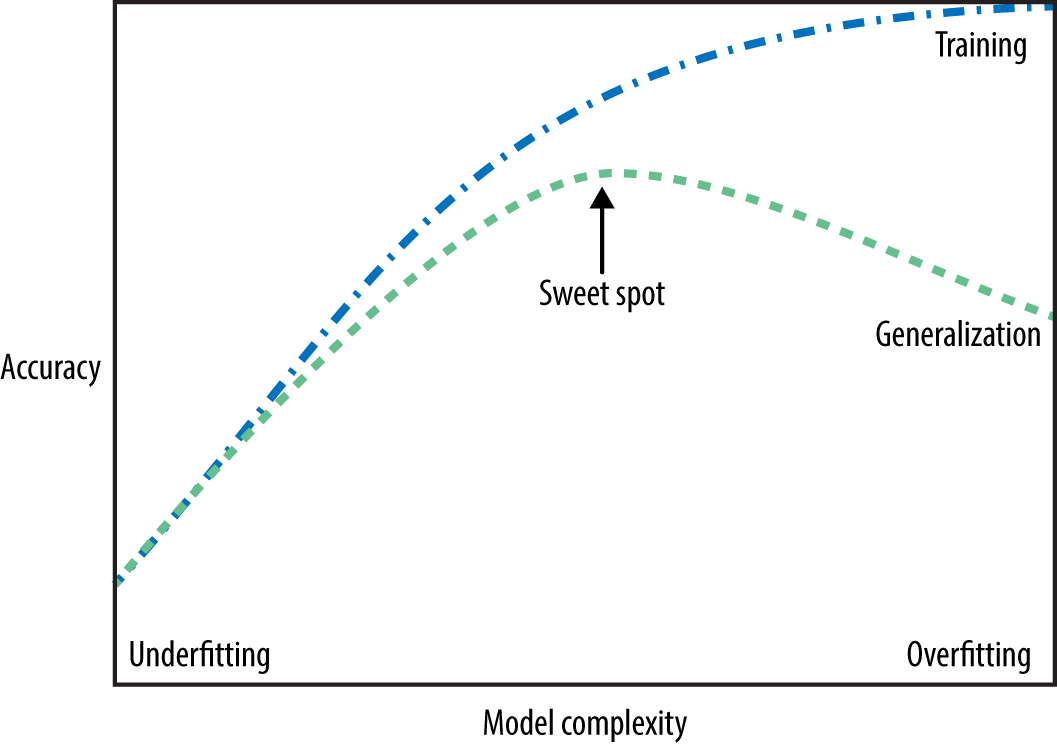
\includegraphics[scale = 0.35]{images/sweet_spot.png}
    \label{fig:sweet_spot}
    \caption{Compromesso tra precisione nella predizione e complessità del modello \cite{figure_copyright}}
\end{figure}


\bigskip
I paragrafi che seguono descrivono nello specifico alcuni algoritmi di apprendimento supervisionato.

\subsubsection{k-Nearest Neighbor}

Il \textit{k-Nearest Neighbor} è un algoritmo utilizzato sia in problemi di classificazione sia in problemi di regressione. 
Questo algoritmo si basa sugli attributi degli oggetti vicini a quello che vogliamo classificare, utilizzando un'opportuna distanza.


\begin{figure}[ht]
    \centering
    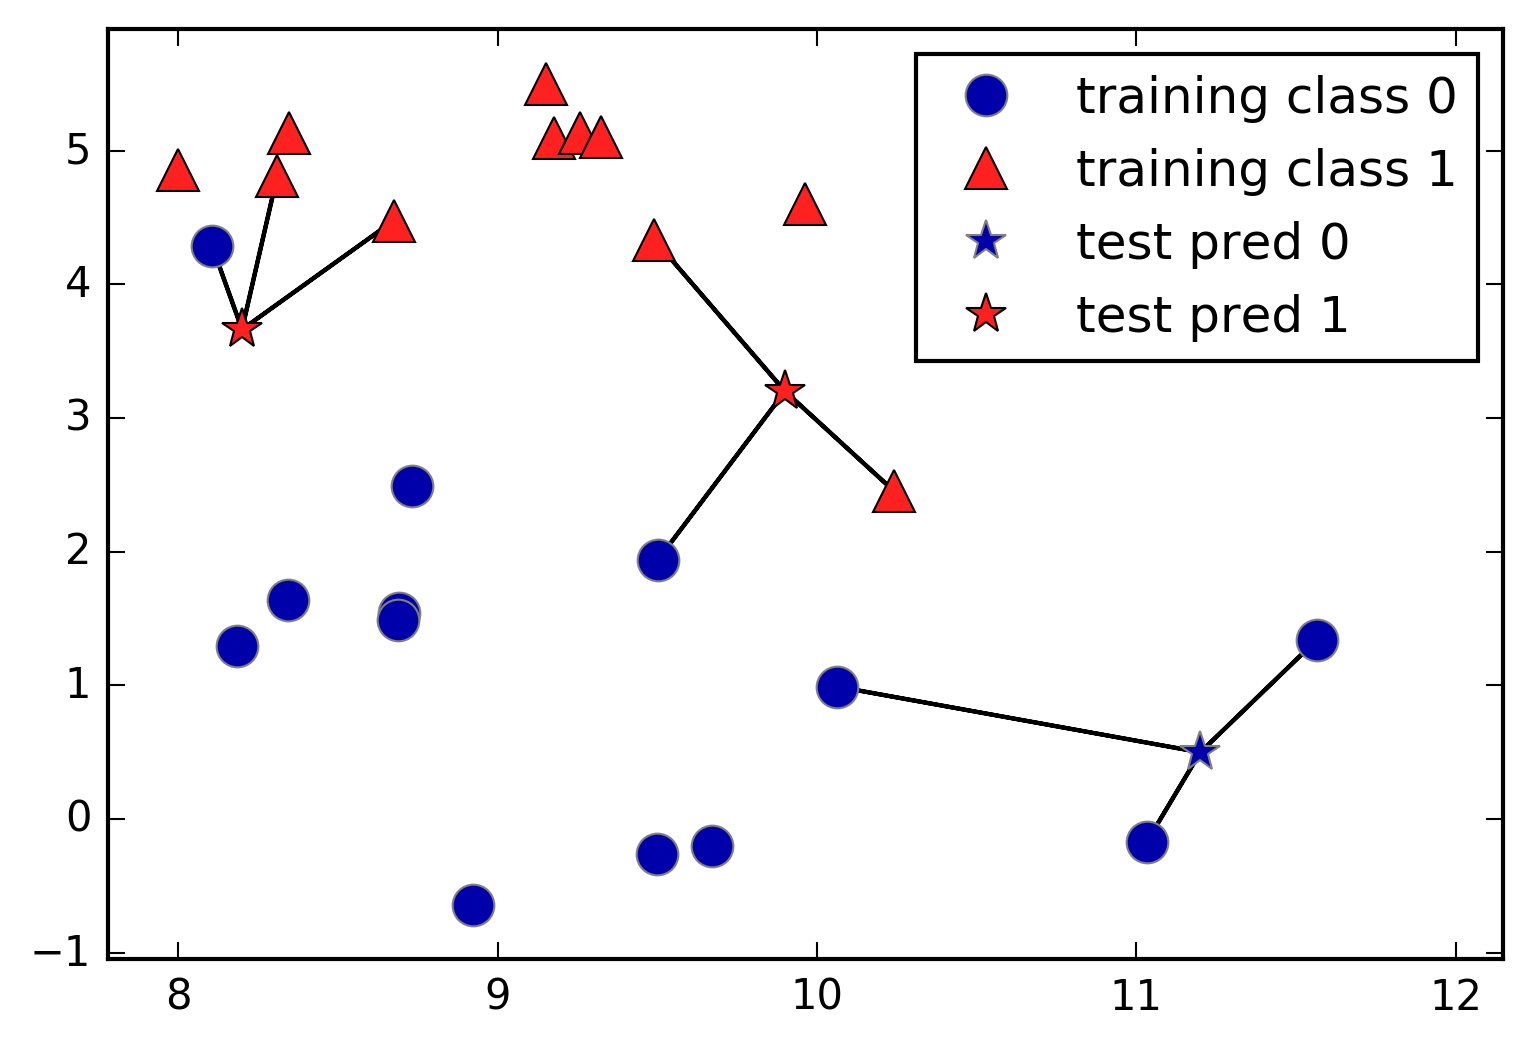
\includegraphics[scale = 0.2]{images/knearest_3_vicini.png}
    \label{fig:knearest_3_vicini}
    \caption{Classificazione tramite k-Nearest Neighbour di 3 elementi. Le stelle rosse rappresentano una classificazione rispetto alla classe 1 (dei triangoli)mentre le stelle blu rappresentano una classificazione rispetto alla classe 0 (dei cerchi) \cite{figure_copyright}.}
\end{figure}


Viene utilizzato un \textit{k} fissato, che indica il numero di vicini da prendere in considerazione per fare la predizione.
La scelta di \textit{k} dipende dalle caratteristiche dei dati. Generalmente all'aumentare di \textit{k} si riduce il rumore che compromette la classificazione, ma il criterio di scelta per la classe diventa più labile.
Questo algoritmo sceglie la classe che occorre maggiormente nei \textit{k} vicini. Infatti nel caso della classificazione binaria è meglio scegliere un \textit{k} dispari per escludere casi di indecisione e quindi poter sempre definire la classe del nuovo dato.

Nel caso di regressione il risultato sarà pari alla media dei valori target dei \textit{k} più vicini.

% come funziona l'algoritmo ? 
% cercare figura che mostri differenza di K
\newpage

\subsubsection{Modelli lineari}
I modelli lineari cercano di effettuare predizioni utilizzando una funzione lineare basata sull'insieme delle caratteristiche dell'elemento da analizzare.

Nel caso della regressione, la funzione è definita come segue: 

\begin{equation*}
    y  = w_0x_0 + w_1x_1 + \dots + w_nx_n + b
\end{equation*}

\noindent dove \textit{n} è il numero di \textit{caratteristiche}, $x_i$ sono le \textit{caratteristiche}, $w_i$ i pesi da attribuire a esse, e $b$ un termine noto.

Quindi il valore $y$ ottenuto applicando la funzione lineare alle caratteristiche di un particolare caso, rappresenta la predzione per l'etichetta corrispondente.

\bigskip

I modelli lineari si possono applicare anche al contesto della classificazione, introducendo degli intervalli sui valori di $y$ per definire a quale classe appartiene il singolo caso. 
Per la classificazione binaria, immaginando di avere due classi, $C_1$ e $C_0$, potremmo avere una formula che associa l'oggetto alla classe $C_0$ se :

\begin{equation*}
    y = w_0x_0 + w_1x_1 + \dots + w_nx_n + b > 0
\end{equation*}

\noindent e alla classe $C_1$ altrimenti.


\subsubsection{Alberi di decisione}

Un albero di decisione (\textit{Decision Learning Tree}) è un modello predittivo utilizzato sia per la classificazione che per la regressione, la cui logica si basa su una struttura ad albero. In quest'ultimo ogni nodo che compare rappresenta una variabile mentre ogni foglia è il risultato finale, ovvero la classe o l'etichetta che volevamo predire per l'oggetto di partenza.

% Un albero di decisione (\textit{Decision Learning Tree}) è un modello predittivo, dove ogni nodo interno rappresenta una variabile, un arco verso un nodo figlio rappresenta un possibile valore per quella proprietà e una foglia il valore predetto per la variabile obiettivo a partire dai valori delle altre proprietà, che nell' albero è rappresentato dal cammino dal nodo radice al nodo foglia.


Nei nodi troviamo delle domande la cui risposta è di tipo binario (vero o falso) mentre le foglie rappresentano le classi che vogliamo predire.

I problemi di \textit{overfitting} e \textit{underfitting} sono problemi ricorrenti che si presentano anche nel caso degli alberi di decisione. Infatti se viene costruito un albero troppo dettagliato, e quindi con un elevato livello di profondità, il modello tende ad adattarsi in maniera eccessiva ai dati usati in fase di allenamento generando un problema di \textit{overfitting}.
Aumentando la profondità dell'albero, infatti, l'errore su un insieme di dati non incluso in quello di allenamento cresce.

Più permettiamo all’albero di avere tanti livelli, più questo ha la capacità di adattarsi meglio ai dati di training, e a partire da una certa lunghezza inizia a farlo a detrimento della sua capacità di generalizzazione. 

Per risolvere questo problema esistono due strategie:
\begin{itemize}
    \item limitare a priori la profondità dell'albero, 
    \item eliminare i nodi che contengono informazioni poco significative.
\end{itemize}

\begin{figure}[ht]
    \centering
    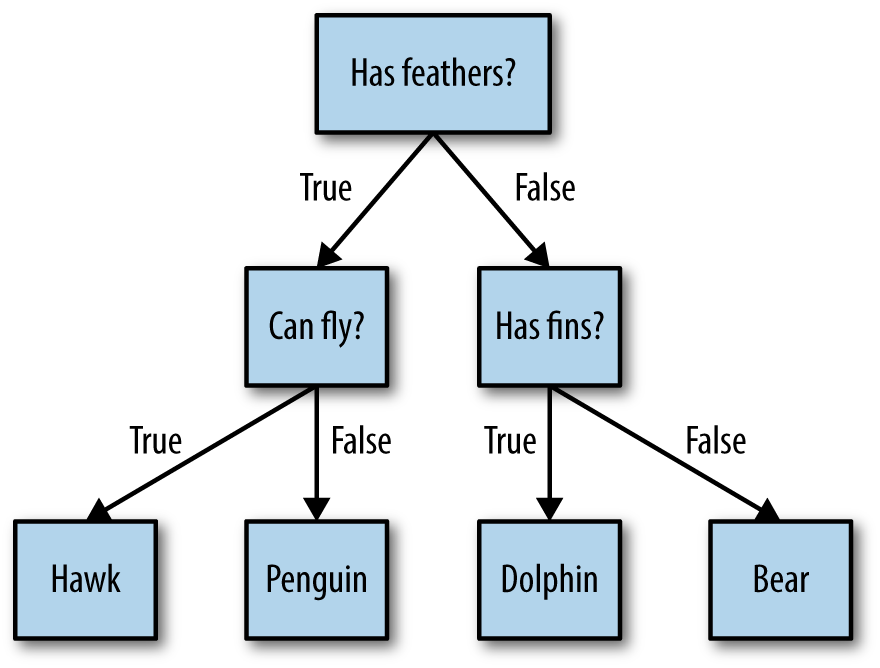
\includegraphics[scale = 0.3]{images/decisione_tree.png}
    \label{fig:decision_tree}
    \caption{Esempio di albero di decisione per la classificazione di un animale. \cite{figure_copyright}}
\end{figure}

\subsubsection{Support Vector Machine}
Le \textit{Support Vector Machine} sono dei modelli di apprendimento utilizzati sia per la regressione che la classificazione.

Una \textit{Support Vector Machine} individua un iperpiano o un insieme di iperpiani per separare i punti in uno spazio e quindi dividerli in diversi gruppi.

Mentre il problema originale può essere definito in uno spazio di dimensioni finite, spesso succede che le classi da distinguere non siano linearmente separabili in quello spazio. Per risolvere questo problema si ricorre alle funzioni \textit{kernel} che sono in grado di mappare dei vettori dallo spazio originale ad uno spazio a dimensionalità più elevata, in cui le immagini risultano separabili.


\subsection*{Approccio Non Supervisionato}
Con \textit{Approccio Non Supervisionato} \cite{unsupervised_learning} ci riferiamo a una tecnica di apprendimento automatico che consiste nel fornire in input una serie di dati non etichettati ma che verranno raggruppati sulla base di caratteristiche comuni  per cercare di effettuare delle previsioni su input futuri.

% L'apprendimento non supervisionato è una tecnica di apprendimento automatico che consiste nel fornire alla macchina una serie di input che verranno riclassificati e organizzati sulla base di caratteristiche comuni per cercare di effettuare ragionamenti e previsioni sugli input successivi. 

Al contrario dell'apprendimento supervisionato, durante l'apprendimento vengono forniti solo esempi non annotati, in quanto le classi non sono note a priori ma devono essere apprese automaticamente.

\bigskip

La principale tecnica in questa categoria è il \textit{clustering}, ovvero una tecnica in grado di suddividere in gruppi distinti  gli oggetti presi in considerazione.

Un esempio di utilizzo ricade nell'ambito della sicurezza informatica. Gli attacchi successivamente rilevati sono probabilmente solo la punta dell'iceberg. Utilizzando tecniche di clustering è possibile individuare e bloccare attacchi ancora sconosciuti.

Il Machine Learning non supervisionato potrebbe utilizzare informazioni dei clienti sugli utilizzi abituali dei servizi di una banca. Se un malintenzionato provasse a effettuare delle operazioni tramite il nostro conto bancario dall'altra parte del mondo a un orario differente da quello abituale, il calcolatore tramite tecniche di clustering, è in grado di riconoscere le operazioni abituali e mandare un messaggio di allarme se individua casi anomali.

\subsection*{Approccio Semi-Supervisionato}
A metà strada tra l'apprendimento supervisionato e quello non supervisionato c'è l'apprendimento semi-supervisionato \cite{supervisedlearning}.

Questo approccio consiste nel combinare le due tecniche e fornire un risultato basandosi su un input eterogeneo costituito da dati etichettati e dati non etichettati.
Questo perché i dati etichettati a volte possono essere difficili, costosi e dispendiosi in termini di tempo e di denaro da recuperare, perché spesso i dati vengono etichettati manualmente da utenti specializzati. Allo stesso tempo i dati non etichettati possono essere relativamente facili da raccogliere, ma ci sono pochi modi di utilizzarli. 
%% Importanza dati non etichettati
L'approccio semi-supervisionato risolve questi problemi utilizzando una grande quantità di dati non etichettati, insieme a una porzione di dati etichettati, per costruire classificatori migliori. 

Ma com'è possibile, avendo a confronto l'apprendimento supervisionato che utilizza solo dati etichettati, avere classificatori migliori tenendo in considerazione i dati non etichettati?
Utilizzando una metafora matematica \cite{supervisedlearning}, potremmo dire che la conoscenza di $p(x)$ che acquisiamo attraverso i dati non etichettati, è un'informazione utile per la predizione di $p(y|x)$. Se non fosse questo il caso, allora non avremo alcun vantaggio rispetto l'apprendimento supervisionato.

\subsection*{Apprendimento con rinforzo}
%%
Il quarto e ultimo approccio, chiamato \textit{Approccio con rinforzo} \cite{Reinforcement_learning}, ha come finalità quella di costruire degli agenti autonomi che hanno il compito di scegliere le azioni da compiere per conseguire determinati scopi attraverso lo studio e l'interazione con il sistema circostante.
In sostanza, utilizzando questo approccio, non siamo noi che istruiamo la macchina, bensì questa decide le azioni da compiere a seconda dello stato attuale del sistema, e così facendo ne determina quello futuro.
%%

Quando la macchina prende una decisione otterrà successivamente una “ricompensa”, sotto forma di punteggio, che sarà alto se la decisione presa è giusta o basso altrimenti. Così l'agente cercherà di fare sempre meglio per arrivare a ottenere il punteggio più alto possibile, prendendo decisioni corrette.

% Link tra insiemi fuzzy e machine learning.

\section{\texorpdfstring{$\mu$}{mu}-learn}
Nel capitolo precedente abbiamo visto le diverse tecniche utilizzate nel Machine Learning. L’algoritmo che andremo a descrivere, denominato \textit{$\mu$-learn}, descritto nel dettaglio nell'articolo \cite{mulearn}, si basa sull’ induzione di insiemi fuzzy e ricade nell’approccio supervisionato, ovvero quella tecnica che necessita di dati preventivamente valutati per effettuare predizioni. In questo caso la predizione è il grado di appartenenza.
\bigskip

Supponiamo di avere un campione {$x_1,\dots,x_m$} in un dominio $X$, ed un insieme di gradi di appartenenza {$\mu_1,\dots,\mu_m$} associati a un generico insieme fuzzy $A$. \newline
Il problema di apprendere $\mu_A$ può essere suddiviso in due parti:
\begin{itemize}
    \item determinare la forma di A;
    \item dedurre i parametri della funzione di membership $\mu_A$
\end{itemize}

\noindent Per fare ciò dobbiamo partire dalle seguenti ipotesi:
\begin{itemize}
    \item L'insieme $A_1 = \{ x\in X \hspace{0,3cm} |\hspace{0,3cm} \mu_A(x) = 1 \}$ deve contenere tutti i punti in $X$ la cui trasformazione attraverso la mappatura $\Phi$ appartenga alla sfera di centro $a$ e raggio $R$.
    
    \item Il grado di appartenenza $\mu_A(x)$ dipende solo dalla distanza tra $\Phi(x)$ e $a$
\end{itemize}

\noindent Fatte queste ipotesi è possibile definire il problema: trovare la più piccola sfera avente centro $a$ e raggio $R$ che includa la maggior parte delle immagini mappate tramite $\Phi$ degli elementi $x\in X$.



La formulazione matematica di questo problema determina un problema di ottimizzazione vincolata, la cui funzione obiettivo è:
\begin{equation*}
    \min R^2 + C\displaystyle\sum_{i=1}^{n}(\xi_i+\tau_i)
    \label{eq:Probela_di_partenza}
\end{equation*}
sottoposta ai seguenti vincoli:
\begin{equation}
    \mu_i\|\Phi(x_i)-a\|^2\le\mu_iR^2 + \xi_i
    \label{eq:vincolo_1}
\end{equation}
\begin{equation}
    (1-\mu_i)\|\Phi(x_i)-a\|^2 \ge (1-\mu_i)R^2 - \tau_i
    \label{eq:vincolo_2}
\end{equation}
\begin{equation}
    \xi_i \ge 0, \tau_i \ge 0
    \label{eq:vincolo_3}
\end{equation}


dove $\xi$ e $\tau$ sono le variabili di scarto utilizzate nel problema di ottimizzazione. $\xi$ è la variabile slack legata al posizionamento dei punti all'interno della sfera, mentre $\tau$ è riferita al posizionamento dei punti all'esterno della sfera. Infine $C$ è una costante la cui funzione è quella di `pesare' l'impatto delle variabili di slack.

Possiamo notare che quando $\mu_i = 1$ otteniamo che il vincolo \ref{eq:vincolo_1} diventa:
\begin{equation*}
    \|\Phi(x_i)-a\|^{2} \le R^2 + \xi_i
\end{equation*}
ovvero che la distanza della trasformazione di $x_i$ da $a$ è minore o uguale al raggio della sfera e che il vincolo \ref{eq:vincolo_2} diventa:
\begin{equation*}
    \tau_i \ge 0
\end{equation*}
che è già incorporato nel vincolo \ref{eq:vincolo_3}, e quindi il nostro $x_i$ sarà posizionato all'interno della sfera.

Allo stesso modo, quando $\mu_i = 0$ otteniamo che il vincolo \ref{eq:vincolo_2} diventa:
\begin{equation*}
    \|\Phi(x_i)-a\|^2 \ge R^2 - \tau_i
\end{equation*}
ovvero che la distanza della trasformazione di $x_i$ da $a$ è maggiore o uguale al raggio della sfera e il vincolo \ref{eq:vincolo_1} così diventa:
\begin{equation*}
    \xi_i \ge 0
\end{equation*}
che è già incorporato nel vincolo \ref{eq:vincolo_3}, e quindi il nostro $x_i$ sarà posizionato all'esterno della sfera.

Utilizzando la formulazione duale di Wolfe, quello che otteniamo è il seguente problema:
\begin{equation}
\begin{split}
    \max \displaystyle\sum_{i=1}^{m}(\alpha_i\mu_i - \beta_i(1-\mu_i))&k(x_i,x_i)\hspace{0,1cm}- \\ &\displaystyle\sum_{i,j=1}^{m}(\alpha_i\mu_i - \beta_i(1-\mu_i))(\alpha_j\mu_j - \beta_j(1-\mu_j))k(x_i,x_j)
\end{split}
\label{eq:problema_finale}
\end{equation}
sottoposto ai vincoli:
\begin{equation}
    \displaystyle\sum_{i=1}^{n}(\alpha_i\mu_i - \beta_i(1-\mu_i)) = 1
    \label{eq:v1_problema_finale}
\end{equation}
\begin{equation}
    0 \le \alpha_i,\beta_i \le C
    \label{eq:v2_problema_finale}
\end{equation}

dove $k$ è la funzione kernel associata alla mappatura nello spazio dell'immagine di $\Phi$ (ovvero $k(x_i,x_j) = \Phi(x_i)\cdot\Phi(x_j))$.

Indicando con $^*$ il valore ottimale per una variabile, è possibile dimostrare che:
\begin{equation*}
\begin{split}
    R^{2}(x) = k(x,x) \hspace{0,1cm}- \hspace{0,1cm}&2\displaystyle\sum_{i=1}^{m}(\alpha{i}^{*}\mu_{i} - \beta_{i}^{*}(1-\mu_{i}))k(x,x_i)\hspace{0,1cm} + \\ 
    &\displaystyle\sum_{i,j=1}^{m}(\alpha_{i}^{*} - \beta_{i}^{*}(1-\mu_{i}))(\alpha_{j}^{*} - \beta_{j}^{*}(1-\mu_{j}))k(x_i,x_j)
\end{split}
\end{equation*}

così facendo è possibile calcolare la distanza tra il centro della sfera e l'immagine del punto dato $x$.
In particolare, tutti i punti $x$ con una membership $\mu_{A}(x) = 1$ soddisfanno $R^2(x) \le R^2_1$ dove $R^2_1 = R^2(x_i)$ per qualunque vettore di supporto.

Apprendere la funzione di membership richiede di trovare il giusto compromesso nella scelta del parametro $C$, così come nei parametri del kernel.




%
%			CAPITOLO 2: tecnologie e metodologie
%

\chapter{Tecnologie e metodologie}
\label{Capitolo 2}
Nel capitolo precendete abbiamo descritto un problema di ottimizzazione vincolata. In questo capitolo vedremo com'è possibile costruirne un'implementazione per la risoluzione.

\bigskip

\noindent Ponendo $\chi_i = (\alpha_i\mu_i - \beta_i(1-\mu_i))$, il problema \ref{eq:problema_finale} può essere riscritto come:
\begin{equation}
    \max \displaystyle\sum_{i=1}^{n}\chi_ik(x_ix_i)\displaystyle\sum_{i,j=1}^{n}\chi_i\chi_j k(x_i,x_j)
\label{eq:problema_finale_2}
\end{equation}

\noindent mentre i vincoli \ref{eq:v1_problema_finale} \ref{eq:v2_problema_finale} diventano:

\begin{equation}
    \displaystyle\sum_{i=1}^{n}\chi_i = 1
    \label{eq:v1_problema_finale_2}
\end{equation}
\begin{equation}
    -C(1-\mu_i) \le \chi_i \le C\mu_i
    \label{eq:v2_problema_finale_2}
\end{equation}

\noindent Come possiamo vedere, grazie a questa manipolazione matematica, quello che otteniamo è un problema di ottimizzazione quadratica vincolato.
Nell'ambito della risoluzione di questo tipo di problema in Python ci sono a disposizione diversi software che permettono di modellare e risolvere il problema.

In particolare la risoluzione di questo problema viene implementata per la parte di ottimizzazione dell'algoritmo \textit{$\mu$-learn} \cite{mulearn_documentation}. Il modulo \textit{optimization} contiente le diverse implementazioni del processo di ottimizzazione dell'induzione dell'insieme fuzzy. In questo modulo è implementata una \textit{Strategy} \cite{strategy_pattern} dove la classe \textit{Solver} è l'interfaccia base che implementa il metodo \textit{solve}, il quale delega il processo di ottimizzazione al metodo astratto \textit{solve\_problem}

\bigskip

\noindent Nei paragrafi successivi vediamo nello specifico come sono stati implementati i solver.

\section{Gurobi}
Gurobi \cite{gurobi} è un software commerciale, disponibile con licenza accademica, utilizzato per la risoluzione di problemi di ottimizzazione. 
Il solver, già disponibile tra gli ottimizzatori della libreria \textit{$\mu$-learn} \cite{mulearn_documentation} 

Cos'è ? Licenza ? Come costruire il problema ? Codice ? 
\section{CVXOPT}
\section{CVXPY}
\section{TensorFlow con Rilassamento Lagrangiano}
\subsection{Rilassamento Lagrangiano}

%
%			CAPITOLO 3: esperimenti fatti

\chapter{Esperimenti}
\label{Captiolo 3}

Spiegare come sono stati costruiti ed eventuali esperimenti
Cercare un filo logico tra gli esperimenti, esperimenti miei e perché li ho fatti così.
\section{Esperimenti a confronto}
\subsection{CVXPY}
\subsection{CVXOPT}
\subsection{TensorFlow}
\subsubsection{Confronto con esperimenti precedenti}

\chapter{Conclusioni}
\label{Conclusioni}

\chapter*{Ringraziamenti}
\label{Ringraziamenti}

%
%			BIBLIOGRAFIA
%

\bibliographystyle{IEEEtran}
\bibliography{biblio}
\addcontentsline{toc}{chapter}{Bibliografia}

\end{document}


 
